\documentclass[12pt,letterpaper]{article}
\usepackage[margin=1in]{geometry}
\usepackage{fancyhdr}
\usepackage[utf8]{inputenc}
\usepackage{palatino}
\usepackage{microtype}
\usepackage{hyperref}
\usepackage{graphicx}
\usepackage{lastpage}
\usepackage[hang,small,margin=1in]{caption}
\usepackage{titlesec}

\renewcommand{\headrulewidth}{0pt}
\fancyfoot{}
\fancyfoot[C]{\sffamily Page \thepage\ of \pageref{LastPage}}
\pagestyle{fancy}

\titleformat{\section}{\bfseries\MakeUppercase}{\arabic{\thesection}}{1em}{}
\titleformat{\subsection}{\bfseries}{\arabic{\thesection}.\arabic{\thesubsection}}{1em}{}
\titleformat{\subsubsection}{\itshape}{\arabic{\thesection}.\arabic{\thesubsection}.\arabic{\thesubsubsection}}{1em}{}

\setlength{\parindent}{0cm}
\setlength{\parskip}{1em}

\captionsetup[figure]{labelfont=it, font=it}
\captionsetup[table]{labelfont={it,sc}, font={it,sc}}

\hypersetup{colorlinks, linkcolor = black, citecolor = black, urlcolor = black}
\urlstyle{same}



\begin{document}

\fancyfoot{}
\begin{center}
  \hfill \\
  \vspace{4in}
  {\bf\Huge CS457 Final Project Proposal:\\Volumetric Smoke\\}
  \vspace{2in}
  {\Large Soo-Hyun Yoo \\ February 20, 2015}
\end{center}

\newpage
\fancyhead{}
\fancyfoot[C]{\sffamily Page \thepage\ of \pageref{LastPage}}

\section*{Final Project Proposal}

In the long term, I would like to take the following steps to implement
procedurally-generated planets with moving, gaseous atmospheres in GLSL:

\begin{enumerate}
  \item {\bf Learn how to render volumes}
  \item {\bf Render volumetric smoke}
  \item {\bf Add 2D and 3D curl noise \cite{bridson07} for smoke}
  \item Animate smoke using curl noise
  \item Implement curl noise smoke on planet
  \item Draw Jupiter's cloud bands and vortices (Figure~\ref{fig:jupiter})
  \item Generate more planets
\end{enumerate}

At least the first three items (in bold) will be implemented for the final
project. Subsequent items will be implemented as time allows.

\begin{figure}[!h]
  \centering
  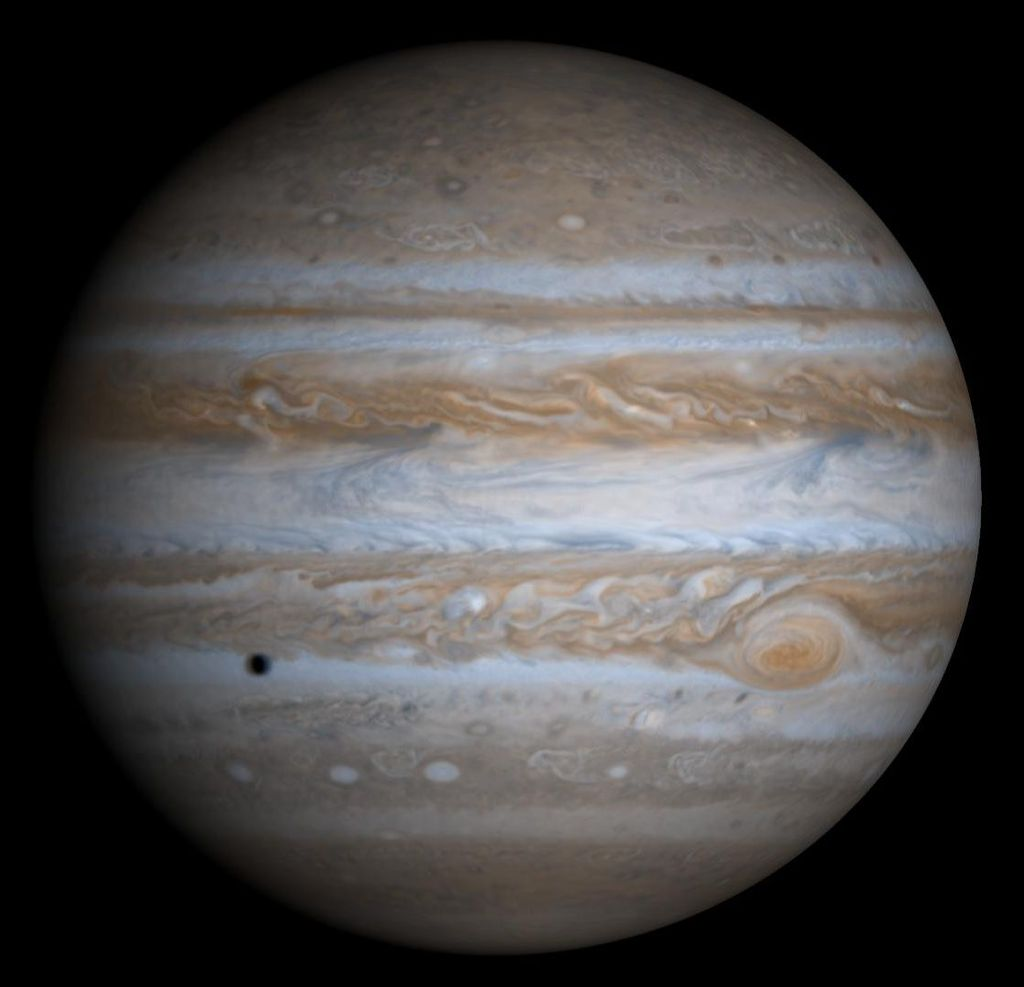
\includegraphics[width=0.5\textwidth]{img/jupiter.jpg}
  \caption{Photo of Jupiter taken by Cassini in 2006.}
  \label{fig:jupiter}
\end{figure}


\begin{thebibliography}{9}
  \bibitem{bridson07} Bridson, Robert, Jim Hourihan, and Marcus Nordenstam. July 2007.
    Curl-Noise for Procedural Fluid Flow. {\it ACM Transactions on Graphics},
    26, 3, Article 46.
\end{thebibliography}

\end{document}
